%----------------------------------------------------------------------------
\appendix
%----------------------------------------------------------------------------
\chapter*{\fuggelek}\addcontentsline{toc}{chapter}{\fuggelek}
\setcounter{chapter}{\appendixnumber}
%\setcounter{equation}{0} % a fofejezet-szamlalo az angol ABC 6. betuje (F) lesz
\numberwithin{equation}{section}
\numberwithin{figure}{section}
\numberwithin{lstlisting}{section}
%\numberwithin{tabular}{section}

%TODO new fugellek here
\newpage
\section{FPGA NES kártya kapcsolási rajza}
\subsection{Tápegység}
\begin{figure}[H]
	\centering
	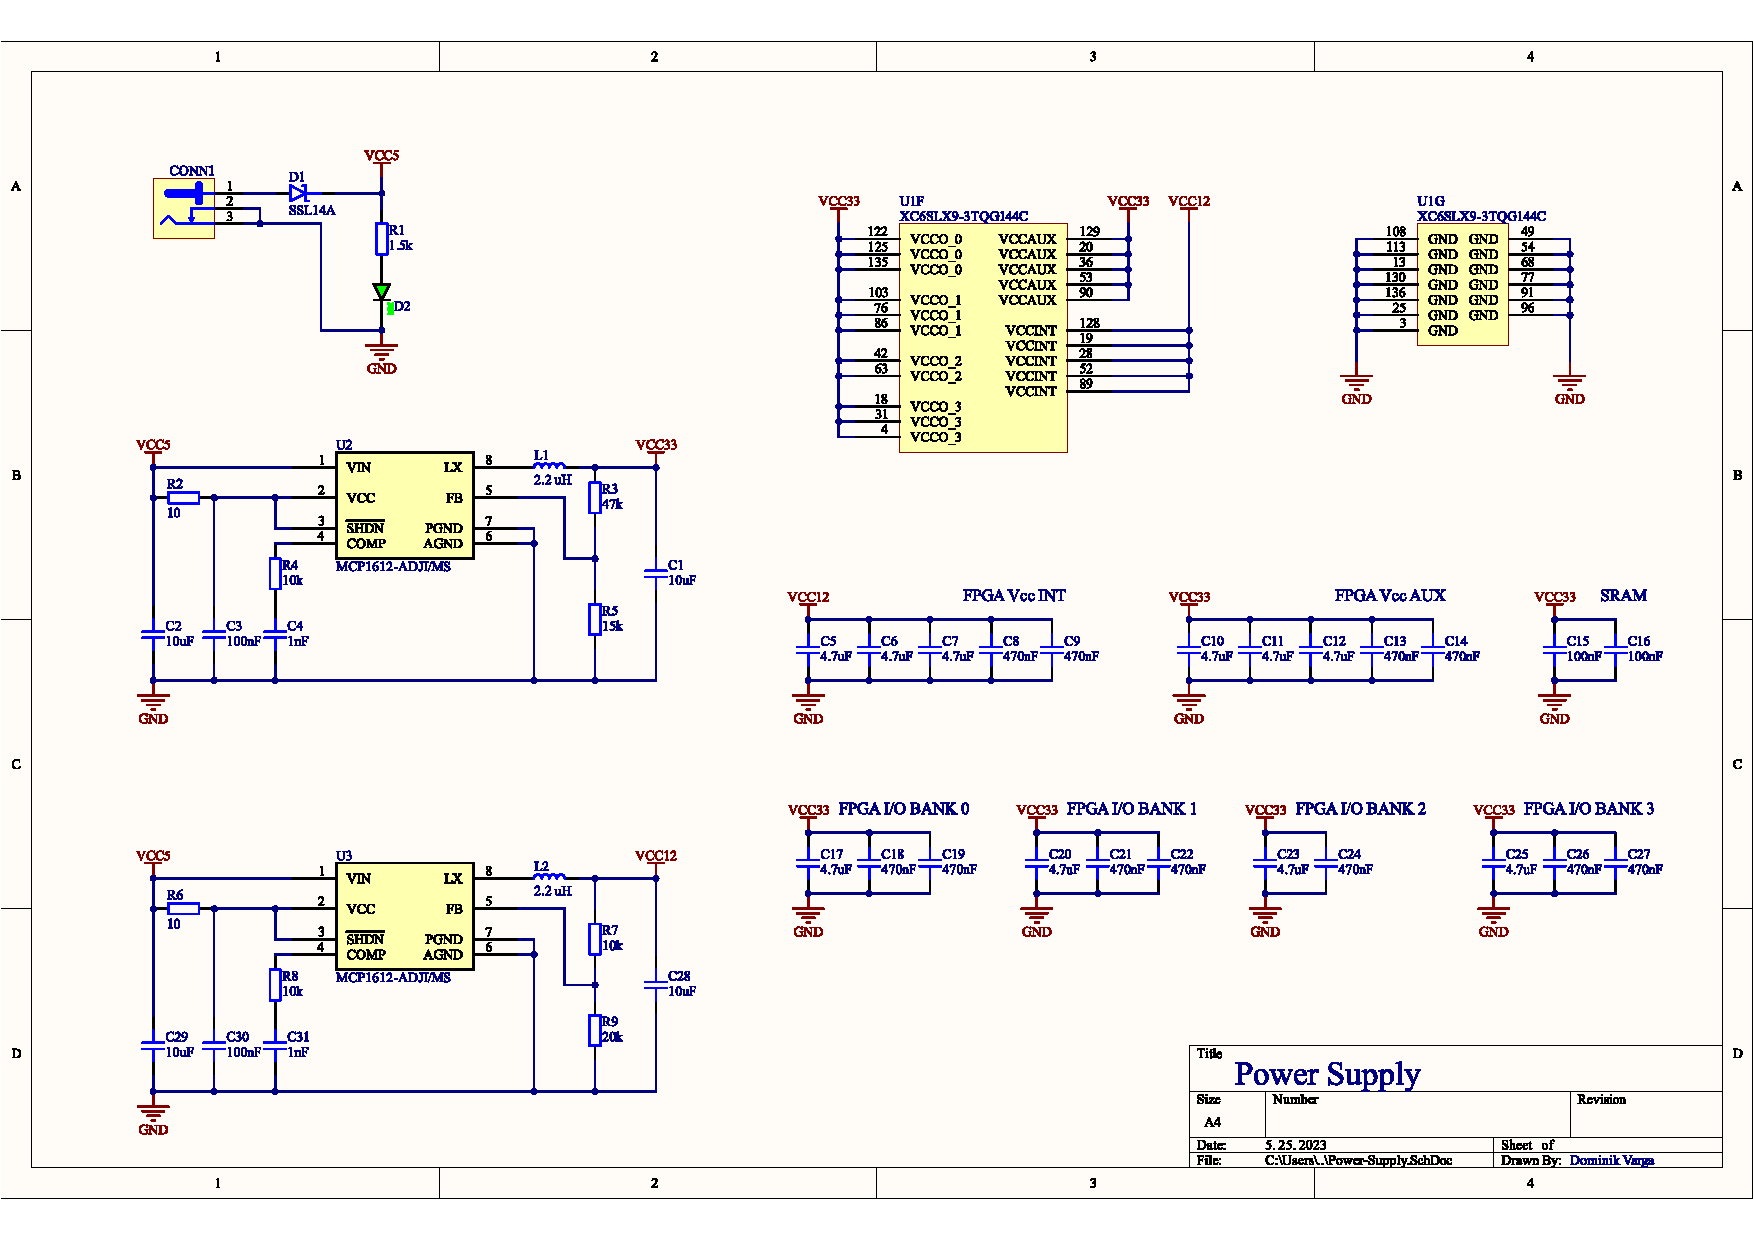
\includegraphics[width=220mm, keepaspectratio, angle=90]{figures/PSU}
	%\caption{Tápegység} 
	\label{fig:PSU}
\end{figure}
\subsection{HDMI és MicroSD kártya csatlakozó}
\begin{figure}[H]
	\centering
	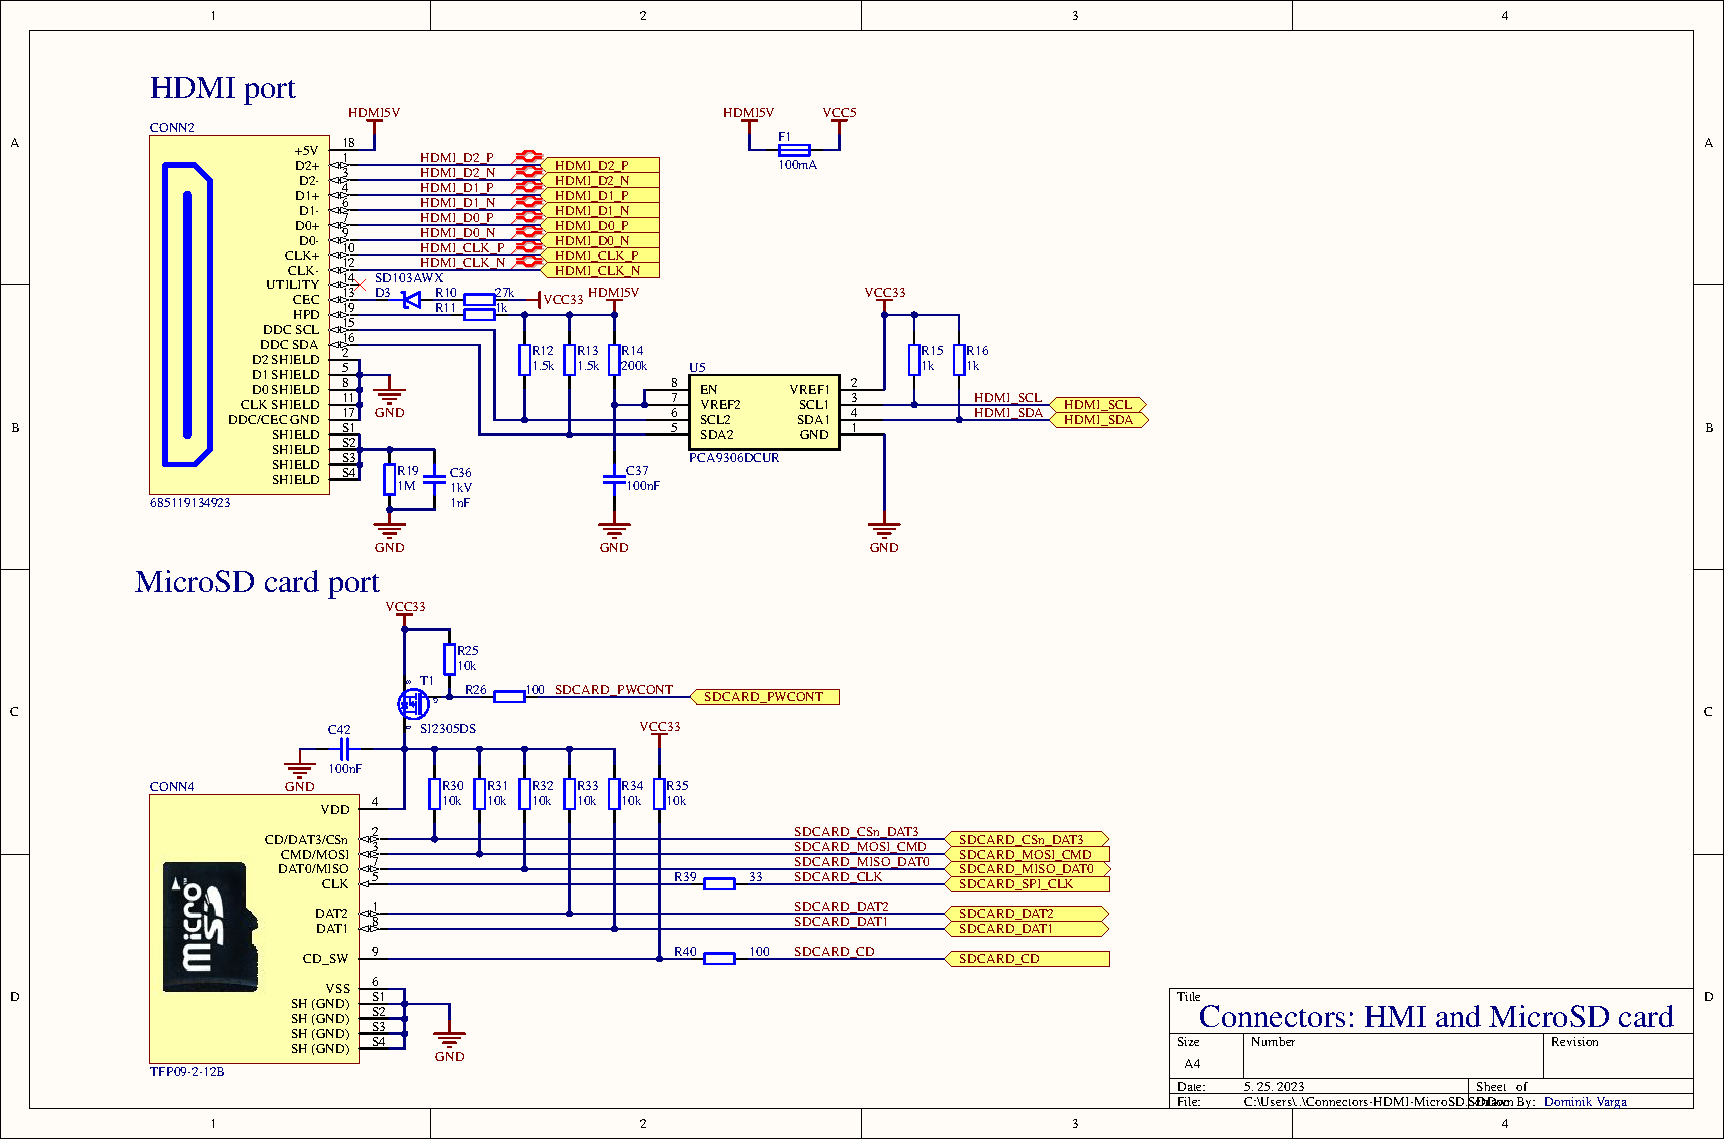
\includegraphics[width=220mm, keepaspectratio, angle=90]{figures/HDMI-MicroSDcard}
	%\caption{HDMI és MicroSD kártya csatlakozó} 
	\label{fig:HDMI-MicroSDcard}
\end{figure}
\subsection{DAC, erősítő és kontroller áramkörök}
\begin{figure}[H]
	\centering
	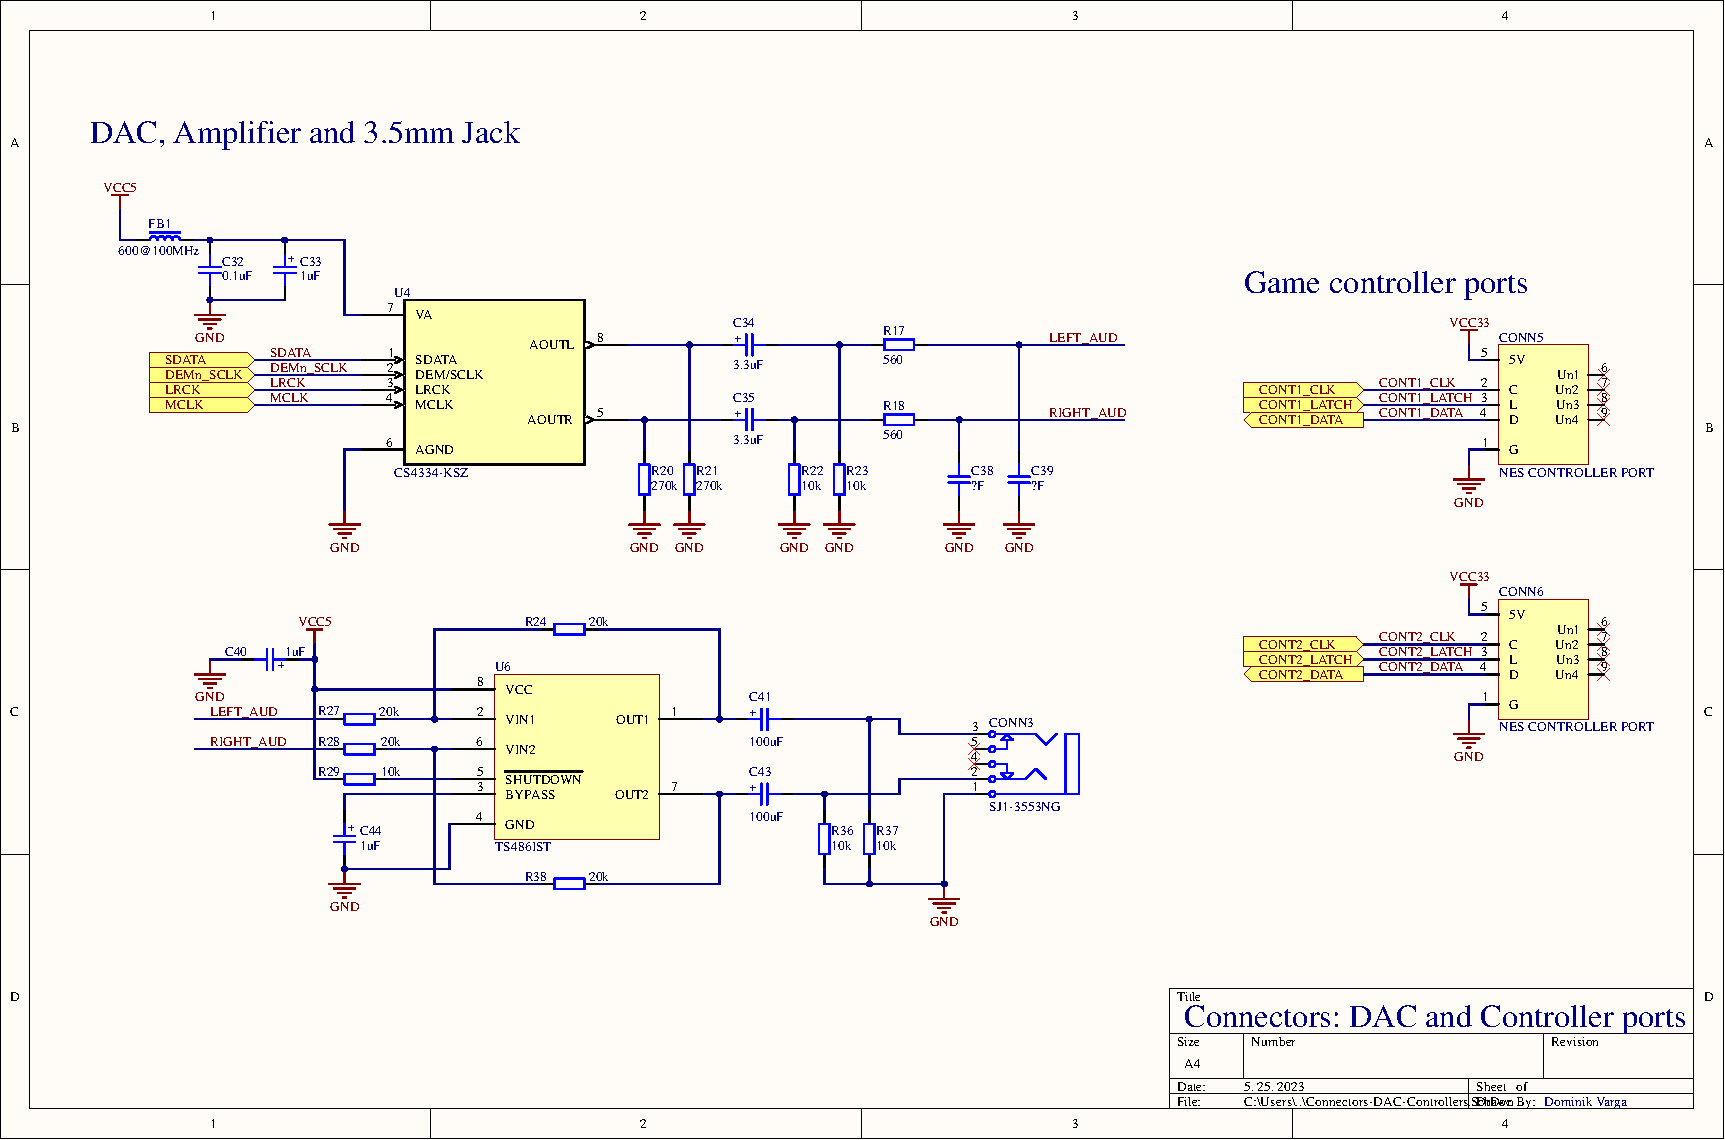
\includegraphics[width=220mm, keepaspectratio, angle=90]{figures/DAC-CONTROLLER}
	%\caption{DAC, erősítő és kontroller áramkörök} 
	\label{fig:DAC-controllers}
\end{figure}
\subsection{SRAM és SPI-Flash}
\begin{figure}[H]
	\centering
	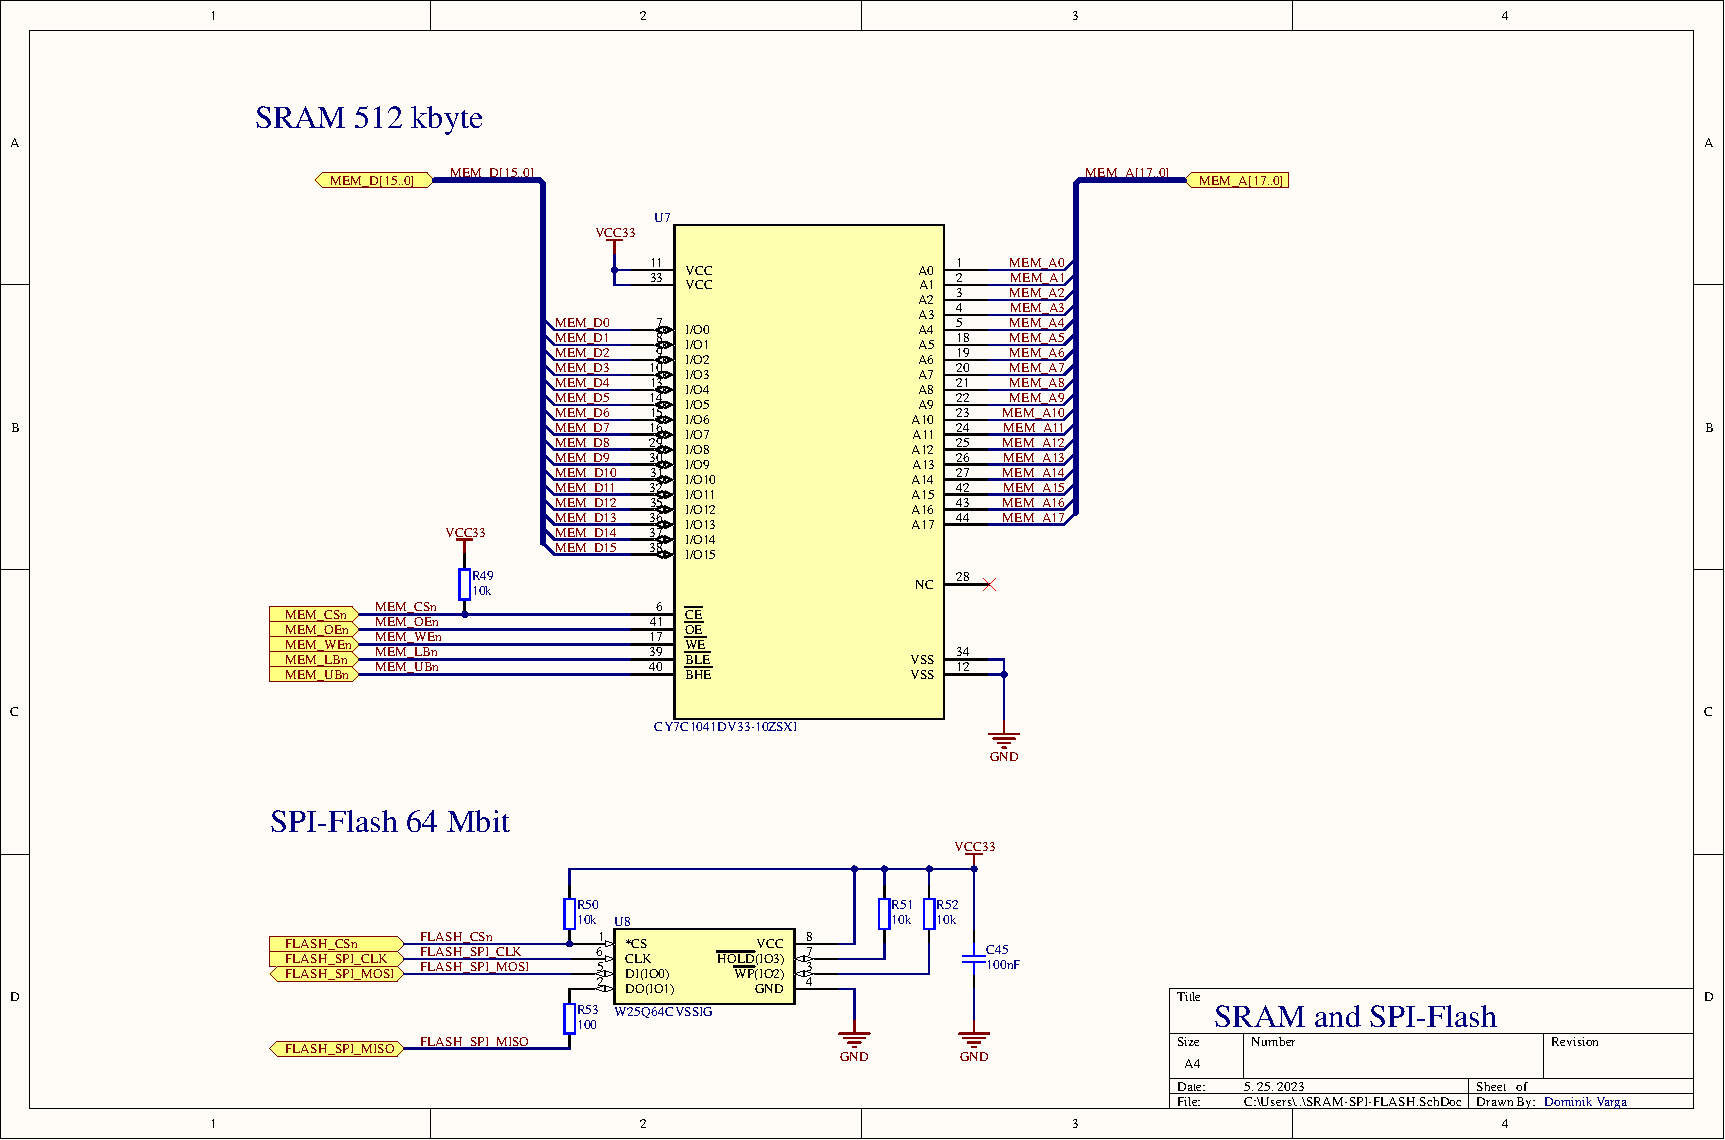
\includegraphics[width=220mm, keepaspectratio, angle=90]{figures/SRAM-FLASH}
	%\caption{SRAM és SPI-Flash} 
	\label{fig:SRAM-SPI-Flash}
\end{figure}
\subsection{FPGA OSC és JTAG}
\begin{figure}[H]
	\centering
	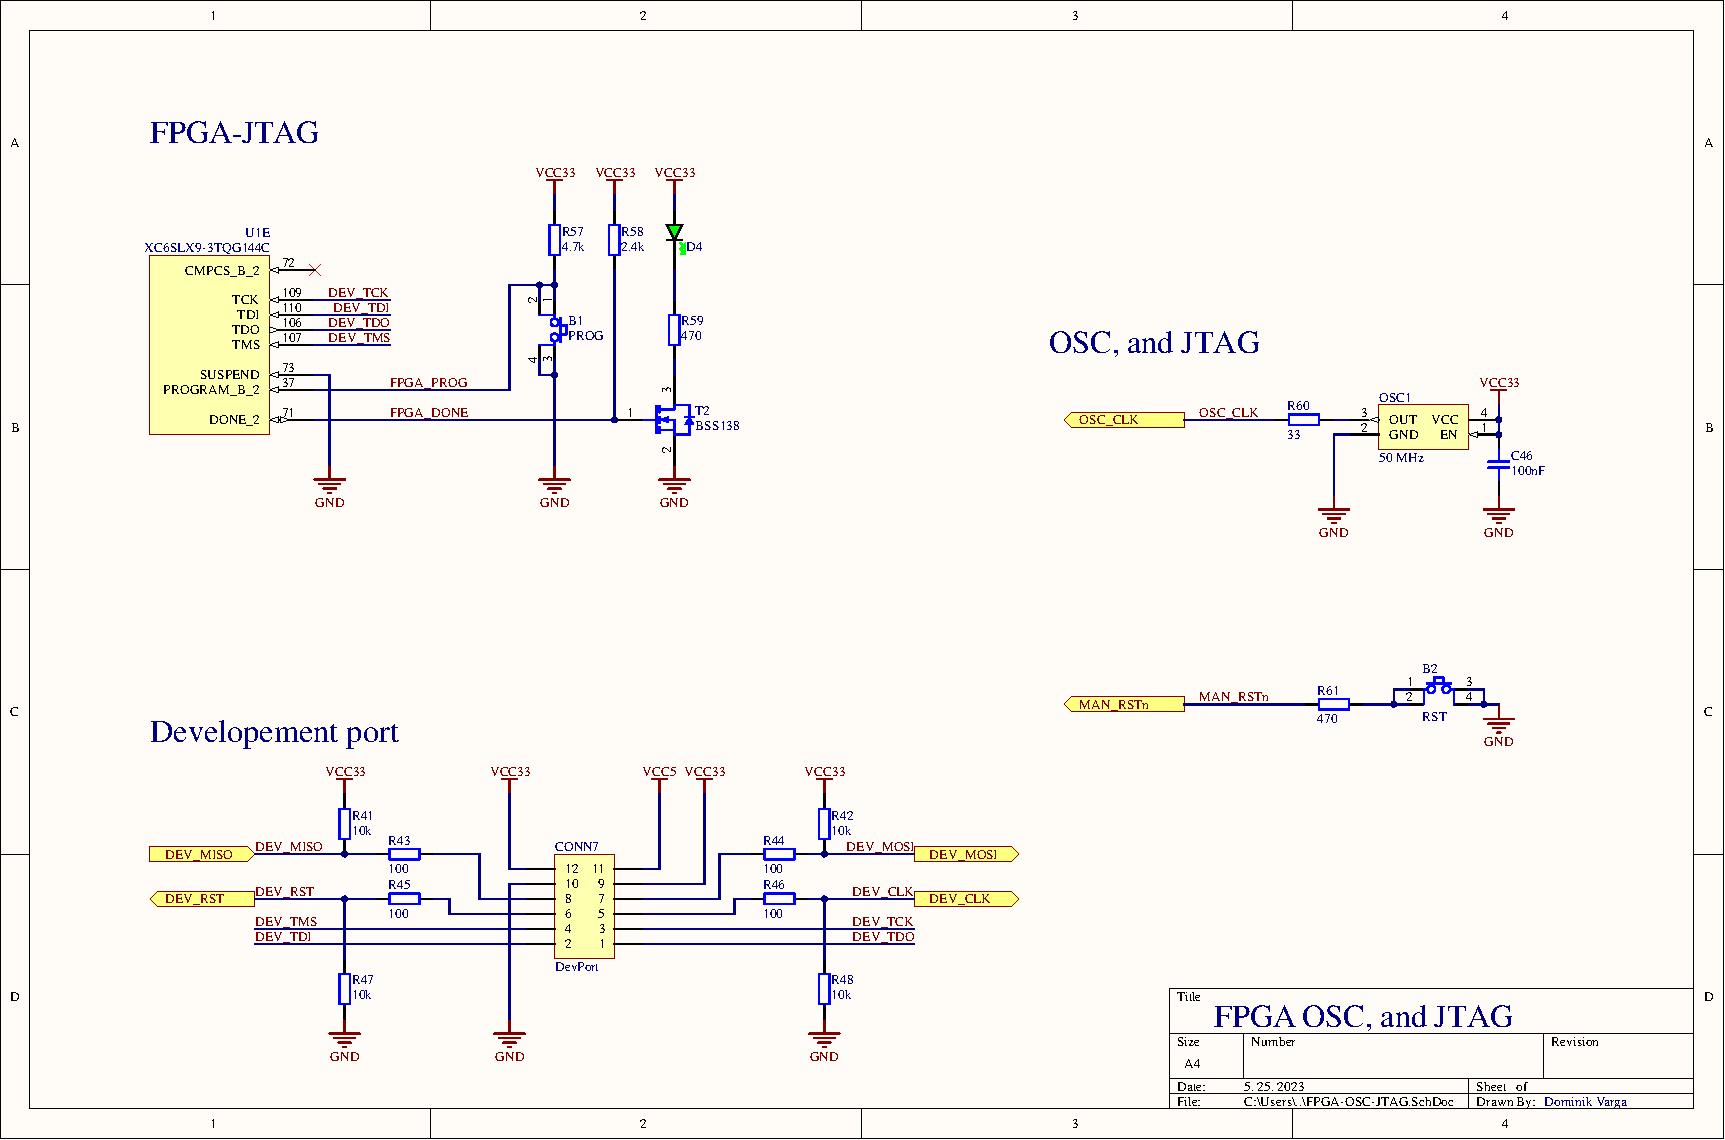
\includegraphics[width=220mm, keepaspectratio, angle=90]{figures/JTAG-OSC}
	%\caption{FPGA OSC és JTAG} 
	\label{fig:OSC-JTAG}
\end{figure}
\subsection{FPGA IO bankok}
\begin{figure}[H]
	\centering
	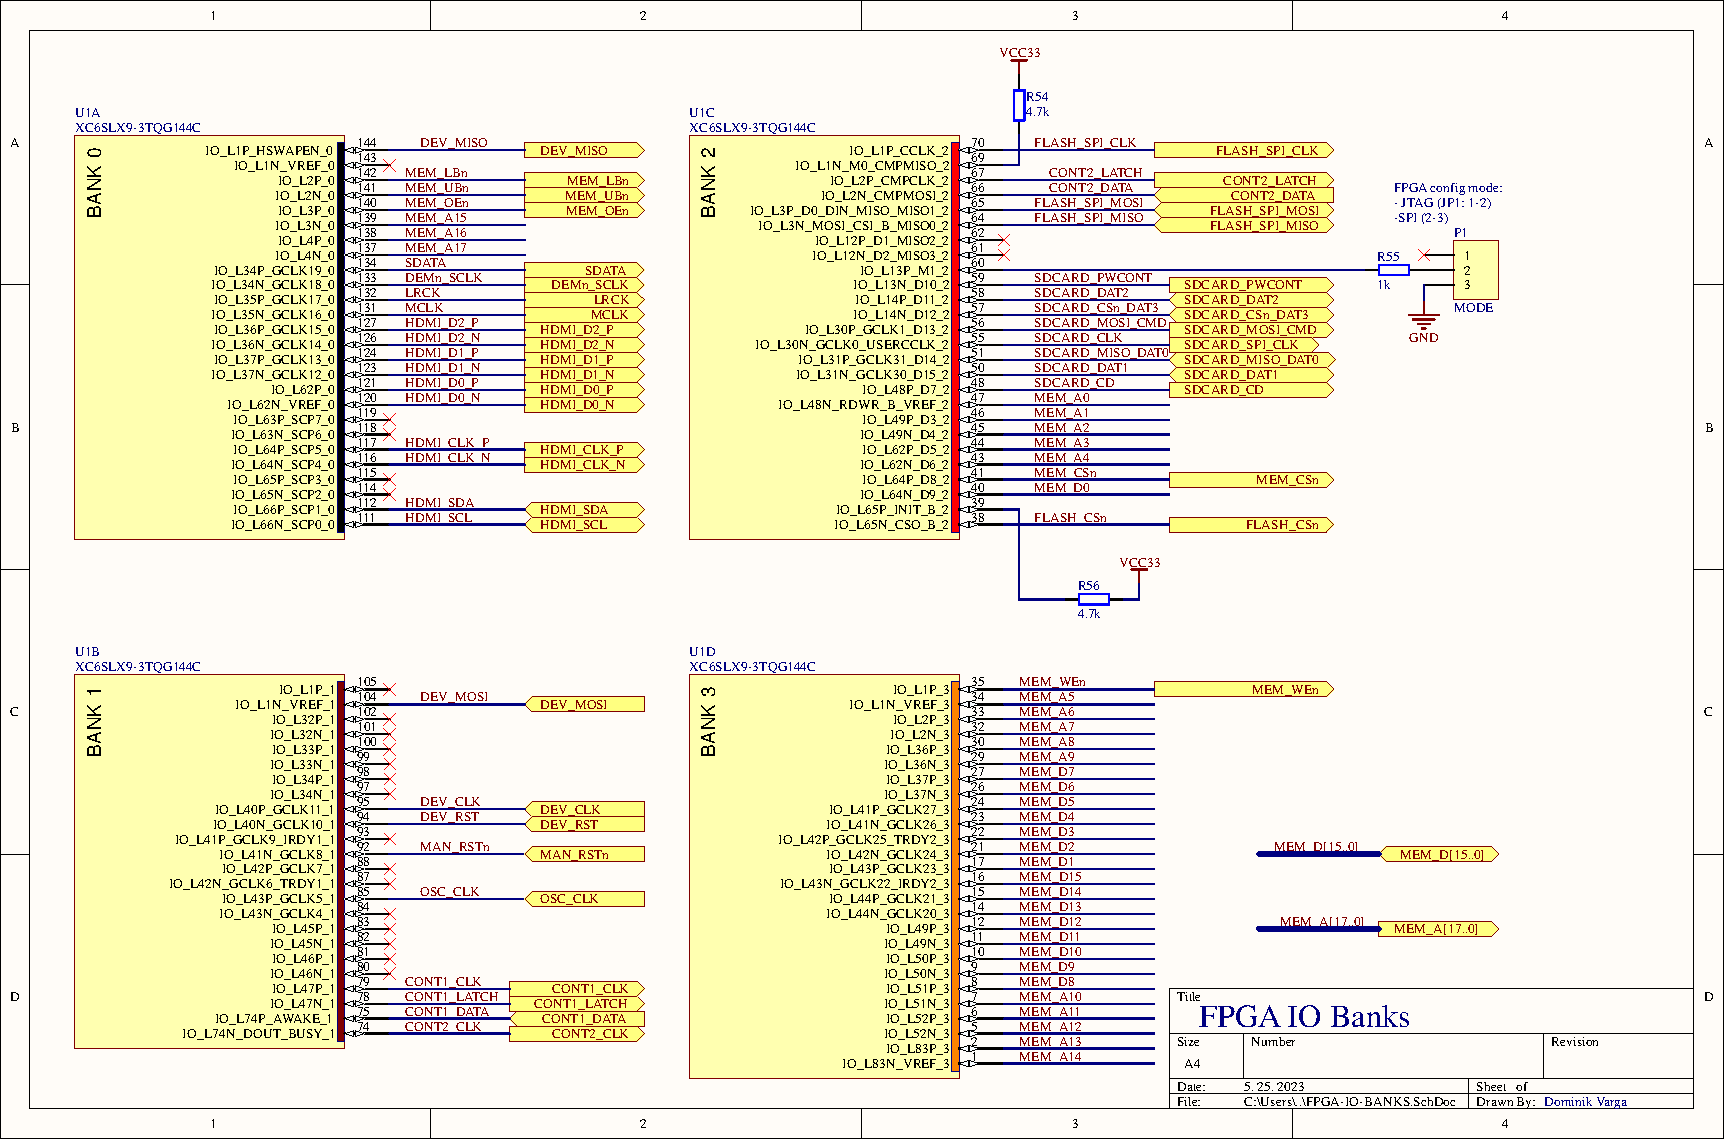
\includegraphics[width=220mm, keepaspectratio, angle=90]{figures/FPGA-BANKS}
	%\caption{FPGA IO bankok} 
	\label{fig:FPGA-BANKS}
\end{figure}
